%polyhedra beeldverwerking
\subsubsection{Beeldverwerking Polyhedra}
{\em Auteur: Laura Vranken ; redactie: Arne Vlietinck}
\\
\\
% eerste stap: splitsen per kleur en binnen/buiten/obstakel
% tweede stap: voor elke kleur de buitenste acht randpunten zoeken
%			   dubbele eruit halen
% derde stap: alleen die overhouden die nog maar 3 hoekpunten hebben (half volledig)
% vierde stap: checken op zwaartepunt overeenkomt
% vijfde stap: linker en rechterbeeld samenvoegen om zwptn te krijgen voor xyz 
% tadaaaaaaaaaaaaaaaa
\noindent
Om naar polyhedra te kunnen vliegen, moet de drone ze eerst kunnen herkennen op de ontvangen beelden. Het analyseren van de beelden gebeurt als volgt. 
\\
Ten eerste worden alle pixels gegroepeerd per kleur. Vervolgens worden de kleuren opgesplitst in verschillende lijsten volgens hun soort, nl. buitendriehoek target, binnendriehoek target of buitendriehoek obstakel. 
\\
Om het zwaartepunt van de driehoek te kunnen bepalen, wordt eerst naar de hoekpunten gezocht. Hiervoor bepalen we voor elke zijde van de driehoek de buitenste pixel. Aangezien het kan zijn dat twee hoekpunten op dezelfde lijn liggen, wordt van elke zijde twee pixels bepaald (de minimum en maximum pixel van de zijde). Op deze manier worden acht pixels gevonden. Figuur \ref{fig:GoedeDriehoek} geeft een voorbeeld van deze methode. Natuurlijk heeft een driehoek geen acht hoeken, dus worden de overeenkomstige buitenste pixels samengenomen tot één hoekpunt. 
\\
Een volledige driehoek behoudt drie hoekpunten. Bovendien kan een driehoek die evenwijdig met een zijde door een andere polyhedra of door de rand van het beeld afgesneden wordt, drie hoekpunten overhouden. Indien niet evenwijdig met een zijde, blijven er vier of meer hoekpunten over. Zie figuur \ref{fig:GoedAfgesnedenDriehoek} voor het eerste geval en figuur \ref{fig:SlechtAfgesnedenDriehoek} voor het tweede geval. Degene met meer dan drie hoekpunten worden niet meer bekeken, ze zijn niet volledig.
\\
Om onderscheid te maken tussen volledige driehoeken en afgesneden driehoeken met drie hoekpunten, wordt de buitendriehoek samen met de overeenkomstige binnendriehoek verder onderzocht. Indien hun zwaartepunten samenvallen, zijn ze volledig. Indien hun zwaartepunten niet samenvallen, kan geconcludeerd worden dat een deel van de driehoek is weggevallen. Zwaartepunten worden bepaald door: \begin{equation}
(x_{zpt},y_{zpt}) = ( \ \frac{1}{3}(x_1 + x_2 + x_3) , \ \frac{1}{3}(y_1 + y_2 + y_3) \ )
\end{equation}
Dit gebeurt voor beide camera's en vervolgens worden de gevonden zwaartepunten gecombineerd en doorgestuurd naar de fysische kant van de Autopilot om omgezet te worden naar 3D coordinaten in het wereldassenstelsel.
\\
\begin{figure}[h]
	\begin{subfigure}{0.33\textwidth}
	\centering
	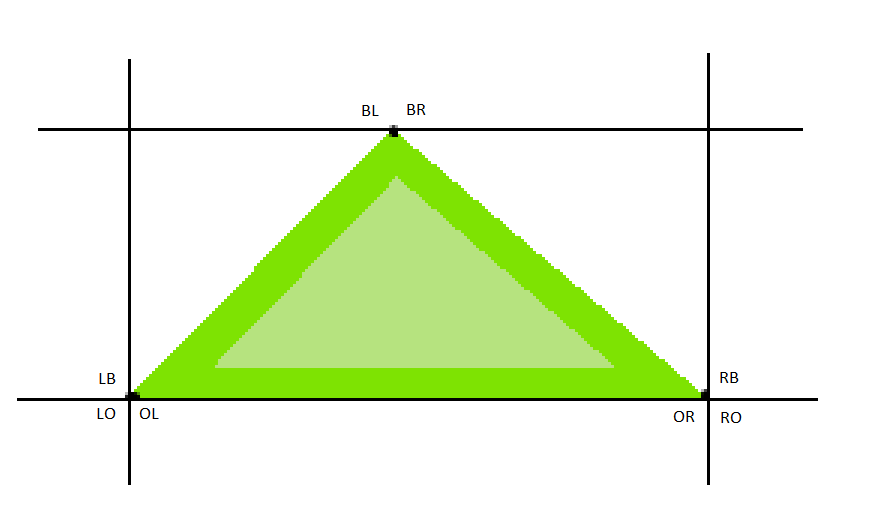
\includegraphics[width=1\textwidth]{GoedeDriehoek.png}
	\caption{Een volledige driehoek.}
	\label{fig:GoedeDriehoek}
	\end{subfigure}
	\begin{subfigure}{0.33\textwidth}
	\centering
	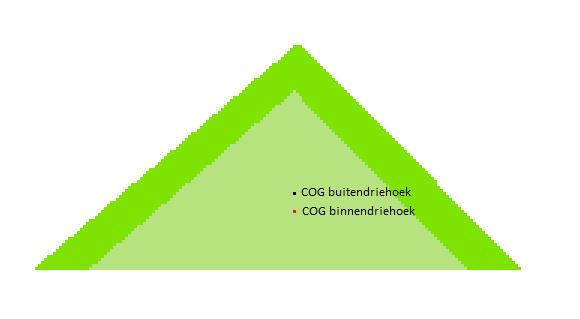
\includegraphics[width=1\textwidth]{GoedAfgesnedenDriehoek.png}
	\caption{Evenwijdig afgesneden driehoek met 3 hoekpunten. De zwaartepunten (COG) liggen echter op een andere plaats.}
	\label{fig:GoedAfgesnedenDriehoek}
	\end{subfigure}
	\
	\begin{subfigure}{0.33\textwidth}
		\centering
		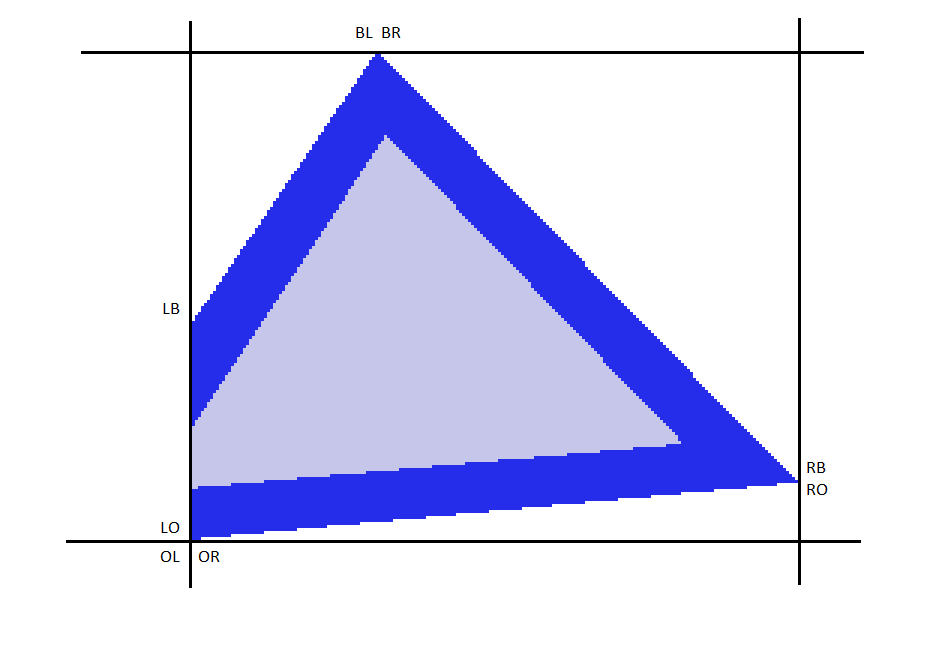
\includegraphics[width=0.9\textwidth]{SlechtAfgesnedenDriehoek.png}
		\caption{Willekeurig afgesneden driehoek met vier hoekpunten.}
		\label{fig:SlechtAfgesnedenDriehoek}
	\end{subfigure}
	\caption{Bepalen van de buitenste 8 punten van mogelijke driehoeken. 
		\\ Afkortingen: LO = links onder, LB = links boven, RO = rechts onder, RB = rechts boven, OL = onder links, OR = onder rechts, BL = boven links, BR = boven rechts.}
	\label{fig:DrieGevallenDriehoeken}
\end{figure}

